\documentclass[
	letterpaper, % Paper size, specify a4paper (A4) or letterpaper (US letter)
	10pt, % Default font size, specify 10pt, 11pt or 12pt
]{CSUniSchoolLabReport}

%----------------------------------------------------------------------------------------
%	REPORT INFORMATION
%----------------------------------------------------------------------------------------

\title{Experiment Five\\ Fundamentals of Electromagnetics Lab \\ EECE2530/1} % Report title

\author{Michael \textsc{Brodskiy}\\ \small \href{mailto:Brodskiy.M@Northeastern.edu}{Brodskiy.M@Northeastern.edu}}

\date{November 8, 2023} % Date of the report

%----------------------------------------------------------------------------------------


\begin{document}

\maketitle % Insert the title, author and date using the information specified above

\begin{center}
	\begin{tabular}{l r}
		Date Performed: & November 1, 2023 \\ % Date the experiment was performed
        Partners: & Manas \textsc{Mahajan} \& Priyam \textsc{Modi} \\ % Partner names
		Instructor: & Professor \textsc{Marengo-Fuentes} \\ % Instructor/supervisor
        TAs: & Nicolas \textsc{Casilli} \& Farah \textsc{Ben Ayed} \\ % Teachers Assistants 
	\end{tabular}
\end{center}

\newpage

\begin{abstract}

  The goal of this laboratory experiment was to test radio transmitters (by implementing a Yagi Uda) and radio receivers, and using the LVDAM-ANT software to record and plot the $\vec{E}$-field and $\vec{B}$-field strength. Various dipole lengths were used to determine the best angle for maximum power transmission.

\end{abstract}

\begin{flushleft}

  \textsc{Keywords:} \underline{transmitter}, \underline{Yagi Uda}, \underline{receiver}, \underline{LVDAM-ANT}, \underline{dipole}, \underline{angle}, \underline{power transmission}

\end{flushleft}

\newpage

\section{Equipment}

\hspace{.5 in} Available equipment included:\\

\begin{itemize}

  \item Yagi Uda Antenna (for transmission)

  \item Dipole Antenna with Modular Length (for receipt)

    \begin{itemize}

      \item Half-Wave Dipole

      \item Full-Wave Dipole

      \item $3/2$-Wave Dipole

    \end{itemize}

  \item LVDAM-ANT Radio Transmission Software

\end{itemize}

\section{Introduction \& Objectives}

We began the experiment by constructing the antennas and choosing the correct lengths for the length of the dipole. As determined in the pre-lab, we began with a half-wave dipole. The antennas were then placed $1[\si{\meter}]$ from each other, at approximately the same height. A radio-frequency generator was then connected and placed in the $1[\si{\kilo\hertz}]$ mode. After connecting all the power supplies and launching the LVDAM-ANT software, the application was able to connect to the receiving antenna.\\

To ensure results that did not oversaturate the antennas, an applicable dB shift was set, and then two measurements was taken. The first measurement recorded the electric field produced by the Yagi Uda (in horizontal orientation), and the second recorded the magnetic field in a similar manner (now vertical orientation). The data acquisition was then repeated for a full-wave and $3/2$-wave dipole.

\section{Results \& Analysis} 

The results for the half-wave dipole are shown in Figures \ref{fig:1}-\ref{fig:4}:

\begin{figure}[H]
  \centering
  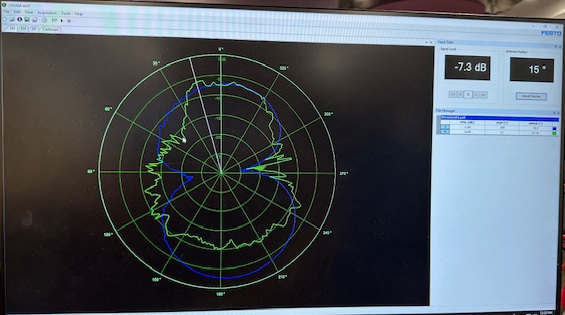
\includegraphics[width=.8\textwidth]{Figures/Lab Five/HWD-Polar.jpg}
  \caption{Half-Wave Dipole Polar Plot}
  \label{fig:1}
\end{figure}

\begin{figure}[H]
  \centering
  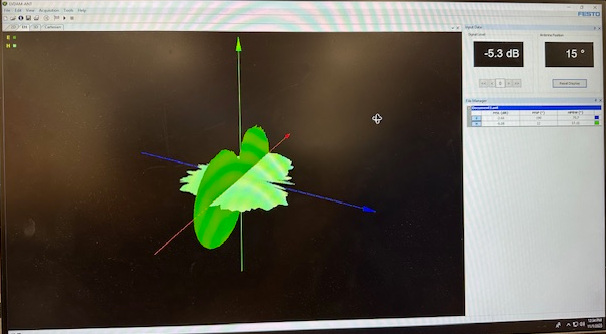
\includegraphics[width=.8\textwidth]{Figures/Lab Five/HWD-2D.jpg}
  \caption{Half-Wave Dipole 2D Plot}
  \label{fig:2}
\end{figure}

\begin{figure}[H]
  \centering
  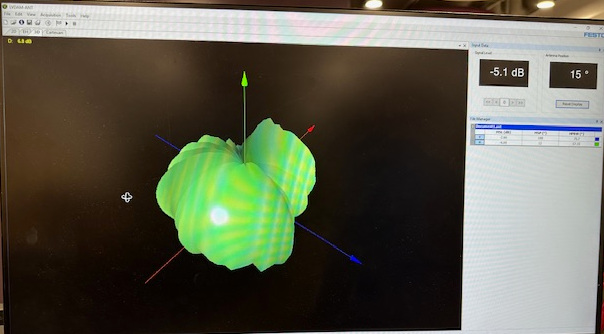
\includegraphics[width=.8\textwidth]{Figures/Lab Five/HWD-3D.jpg}
  \caption{Half-Wave Dipole 3D Plot}
  \label{fig:3}
\end{figure}

\begin{figure}[H]
  \centering
  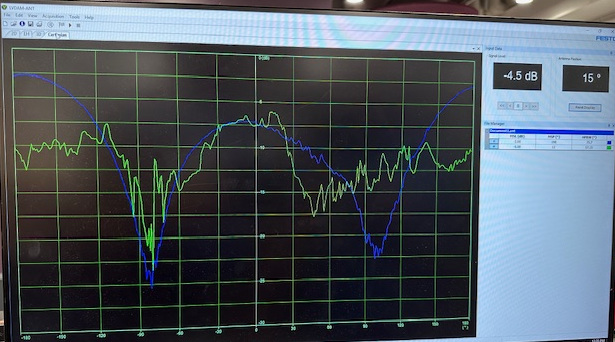
\includegraphics[width=.8\textwidth]{Figures/Lab Five/HWD-XY.jpg}
  \caption{Half-Wave Dipole Cartesian Plot}
  \label{fig:4}
\end{figure}

The results for the full-wave dipole are shown in Figures \ref{fig:5}-\ref{fig:8}:

\begin{figure}[H]
  \centering
  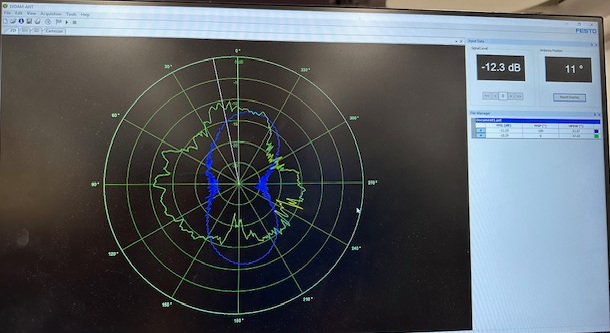
\includegraphics[width=.8\textwidth]{Figures/Lab Five/FWD-Polar.jpg}
  \caption{Full-Wave Dipole Polar Plot}
  \label{fig:5}
\end{figure}

\begin{figure}[H]
  \centering
  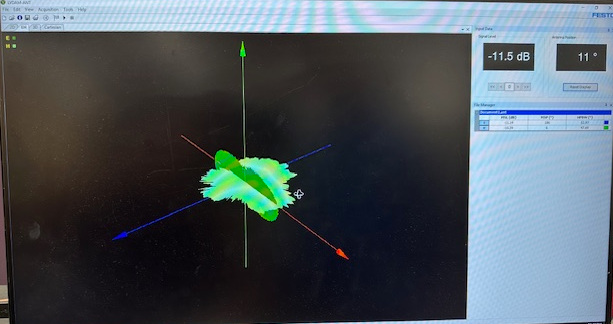
\includegraphics[width=.8\textwidth]{Figures/Lab Five/FWD-2D.jpg}
  \caption{Full-Wave Dipole 2D Plot}
  \label{fig:6}
\end{figure}

\begin{figure}[H]
  \centering
  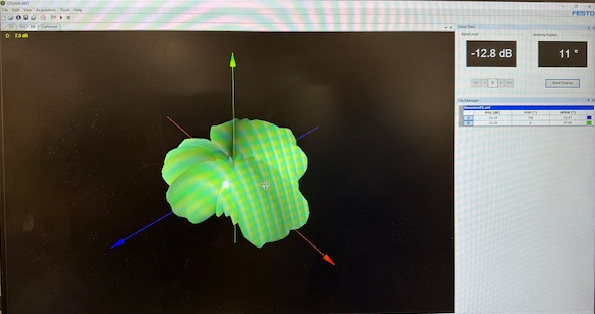
\includegraphics[width=.8\textwidth]{Figures/Lab Five/FWD-3D.jpg}
  \caption{Full-Wave Dipole 3D Plot}
  \label{fig:7}
\end{figure}

\begin{figure}[H]
  \centering
  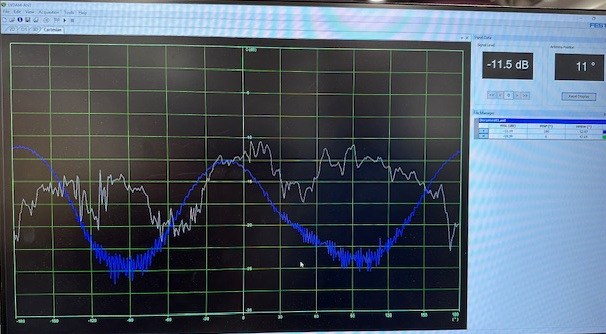
\includegraphics[width=.8\textwidth]{Figures/Lab Five/FWD-XY.jpg}
  \caption{Full-Wave Dipole Cartesian Plot}
  \label{fig:8}
\end{figure}

The results for the $3/2$-wave dipole are shown in Figures \ref{fig:9}-\ref{fig:12}:

\begin{figure}[H]
  \centering
  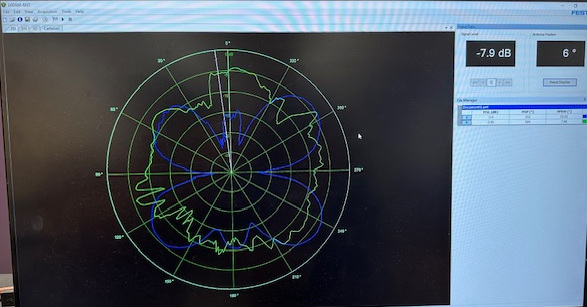
\includegraphics[width=.8\textwidth]{Figures/Lab Five/3-2WD-Polar.jpg}
  \caption{$3/2$-Wave Dipole Polar Plot}
  \label{fig:9}
\end{figure}

\begin{figure}[H]
  \centering
  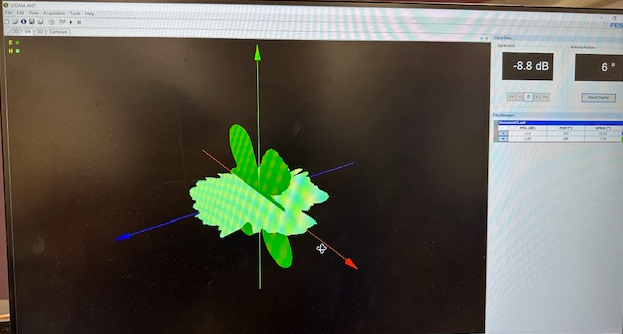
\includegraphics[width=.8\textwidth]{Figures/Lab Five/3-2WD-2D.jpg}
  \caption{$3/2$-Wave Dipole 2D Plot}
  \label{fig:10}
\end{figure}

\begin{figure}[H]
  \centering
  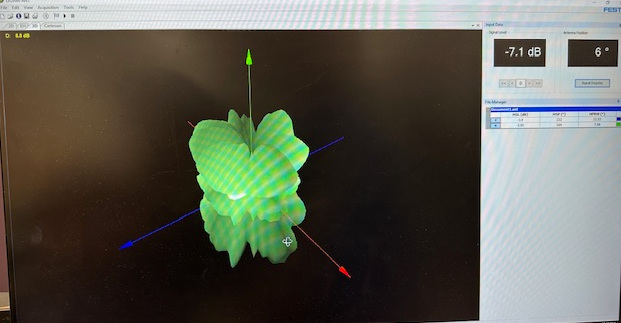
\includegraphics[width=.8\textwidth]{Figures/Lab Five/3-2WD-3D.jpg}
  \caption{$3/2$-Wave Dipole 3D Plot}
  \label{fig:11}
\end{figure}

\begin{figure}[H]
  \centering
  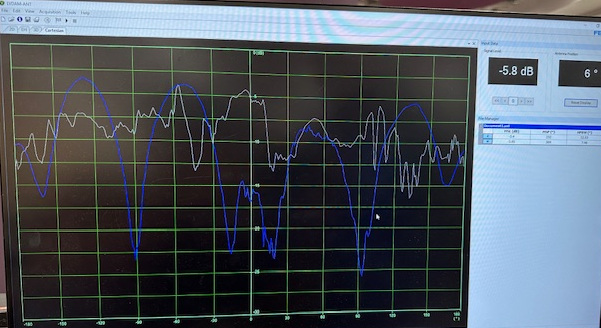
\includegraphics[width=.8\textwidth]{Figures/Lab Five/3-2WD-XY.jpg}
  \caption{$3/2$-Wave Dipole Cartesian Plot}
  \label{fig:12}
\end{figure}

\section{Conclusion}

\subsection{Questions}

\begin{enumerate}

  \item Compare the patterns of the antenna you measured. Did they receive the same power? Please comment referring to the measured data.

    The Festo results seem to be in much more idealized conditions, most likely taken in an anechoic chamber. Comparing this to our graphs, we can see that we received a similar level of power; however, our results experienced much more reflective interference. We know this because the results should be much smoother, whereas, especially with respect to our magnetic field graphs, the results feature many sharp points. In addition to reflective interference, this could have been a result of the clutter of similar experiments being performed close to us.

  \item Evaluate the input impedance of the antennas with the presented formulas.

    We know from our formulas that:

    $$R_{in}=R_{rad}+R_{loss}$$

    However, for a dipole as effective as this, we can assume $R_{loss}$ is small enough to ignore. Thus, this gives us:

    $$R_{in}=R_{rad}=80\pi^2\left( \frac{l}{\lambda} \right)^2$$

    This gives us the three input resistances as:

    $$R_{in}=\left\{\begin{array}{l l l} l=.5\lambda, & 20\pi^2 &=197.39[\si{\ohm}]\\ l=\lambda, & 80\pi^2 &=789.57[\si{\ohm}]\\l=1.5\lambda, & 180\pi^2 &=1.776[\si{\kilo\ohm}]\end{array}$$

  \item Evaluate the HPBW for the antennas.

    Though it is difficult to see in the images above, the HPBW can be tabulated as follows:

    \begin{center}
      \begin{tabular}[h]{|c|c|c|}
        \hline
        Dipole Length [$\si{\meter}$] & Electric HPBW ($^{\circ}$) & Magnetic HPBW ($^{\circ}$)\\
        \hline
        $l=.5\lambda$ & 75.7 & 57.15\\
        \hline
        $l=\lambda$ & 52.97 & 47.69\\
        \hline
        $l=1.5\lambda$ & 32.52 & 7.98\\
        \hline
      \end{tabular}
    \end{center}

    As expected, we can see that, as the dipole gets wider, the HPBW decreases. Essentially, this means that the field is most effectively transmitted within this angle of the dipole. Thus, we know that a larger dipole would receive a more directed field, which is indicated by the data.

  \item What if we rotate the Yagi and transmit with the dipole? What do you expect to see?

    In general, a Yagi Uda is better a transmission, while a dipole is better at receipt. Thus, in reversing the roles, we would expect the radiation to be less directed. This would mean the HPBW values would increase, which would indicate less power arriving at the Yagi Uda. As such, we would expect to see a weaker field with a greater HPBW.

  \item Why is the Yagi a good antenna to test other antennas?

    Yagi Uda antennas are good because of their high directionality. Because of the structure, the produced field is generally well-directed, allowing for greater power transmission in a certain direction, as evident by the fairly low HPBW values. As such, because they are capable of directing their signals better than other antennas, it is easier to test receivers.

\end{enumerate}

\subsection{Summary}

Overall, we were able to successfully generate all of the necessary plots and data from testing the antennas. It is visible for nearly all of the plots, however, that significant reflections interfered with some of the transmissions.

\end{document}
